\documentclass[presentation,handout]{beamer}
\usepackage[utf8]{inputenc}
\usepackage[T1]{fontenc}
\usepackage{graphicx}
\usepackage{grffile}
\usepackage{longtable}
\usepackage{wrapfig,epigraph}
\usepackage{rotating}
\usepackage[normalem]{ulem}
\usepackage{amsmath}
\usepackage{textcomp}
\usepackage{amssymb}
\usepackage{capt-of}
\usepackage{hyperref, tipa}
\let\pb\relax

\usepackage{tikz}
\usetikzlibrary{calc}
\makeatletter
\def\th@mystyle{%
    \normalfont % body font
    \setbeamercolor{block title example}{bg=red!5,fg=red!65!black}
    \setbeamercolor{block body example}{ bg=red!5,fg=black}
    \def\inserttheoremblockenv{exampleblock}
  }
\makeatother

\newcommand{\xto}[1]{\xrightarrow{#1}}
\newcommand{\xot}[1]{\xleftarrow{#1}}

\theoremstyle{mystyle}
	\newtheorem{df}{Definition}
	\newtheorem{oss}{Remark}
	\newtheorem{cor}{Corollary}
	\newtheorem{thm}{Theorem}
	\newtheorem{prop}{Proposition}
	\newtheorem{es}{Example}

\def\yo{y}
\def\shape{\text{\textesh}}
\def\thH{\widetilde{\clH}}
\def\disc{\textsc{disc}}
\def\codisc{\textsc{codisc}}

\usepackage{xparse}
\usepackage[color,all,2cell]{xy}\UseAllTwocells

\colorlet{dagreen}{green!70!black}

\def\quadruple#1{%
	\ar@<12pt>@{^{(}->}[r]%
	\ar@{<-}@<4pt>[r]|{i^*_{#1}}%
	\ar@<-4pt>@{^{(}->}[r]|{i_{*,#1}}%
	\ar@<-12pt>@{<-}[r]%
 }

\ExplSyntaxOn
\NewDocumentCommand{\makeabbrev}{mmm}
 {
  \yoruk_makeabbrev:nnn { #1 } { #2 } { #3 }
 }

\cs_new_protected:Npn \yoruk_makeabbrev:nnn #1 #2 #3
 {
  \clist_map_inline:nn { #3 }
   {
    \cs_new_protected:cpn { #2 } { #1 { ##1 } }
   }
 }
\ExplSyntaxOff

\makeabbrev{\textbf}{bf#1}{
  a,b,c,d,e,g,h,i,j,k,l,m,n,o,p,q,r,t,u,v,w,x,y,z,%
  A,B,C,D,E,G,H,I,J,K,L,M,N,O,P,Q,R,T,U,V,W,X,Y,Z }
\makeabbrev{\boldsymbol}{bs#1}{%
    a,b,c,d,e,f,g,h,i,j,k,l,m,n,o,p,q,r,s,t,u,v,w,x,y,z,%
    A,B,C,D,E,F,G,H,I,J,K,L,M,N,O,P,Q,R,S,T,U,V,W,X,Y,Z }
\makeabbrev{\mathsf}{sf#1}{
  a,b,c,d,e,f,g,h,i,j,k,l,m,n,o,p,q,r,s,t,u,v,w,x,y,z,%
  A,B,C,D,E,F,G,H,I,J,K,L,M,N,O,P,Q,R,S,T,U,V,W,X,Y,Z }
\makeabbrev{\mathfrak}{fk#1}{
  a,b,c,d,e,f,g,h,j,k,i,l,m,n,o,p,q,r,s,t,u,v,w,x,y,z,%
  A,B,C,D,E,F,G,H,I,J,K,L,M,N,O,P,Q,R,S,T,U,V,W,X,Y,Z }
\makeabbrev{\mathcal}{cl#1}{
  A,B,C,D,E,F,G,H,I,J,K,L,M,N,O,P,Q,R,S,T,U,V,W,X,Y,Z }
\makeabbrev{\mathbb}{bb#1}{
  A,B,C,D,E,F,G,H,I,J,K,L,M,N,O,P,Q,R,S,T,U,V,W,X,Y,Z }

\newlength{\seplen}
\setlength{\seplen}{5pt}
\newlength{\sepwid}
\setlength{\sepwid}{.4pt}
\def\firstblank{\,\rule{\seplen}{\sepwid}\,}
\def\secondblank{\firstblank\llap{\raisebox{2pt}{\firstblank}}}
\def\To{\Rightarrow}

\def\Set{\underline{\text{Set}}}
\newcommand{\op}{\text{op}}

\setbeamertemplate{navigation symbols}{}
\usepackage{animate}

\newenvironment{variableblock}[3]{%
  \setbeamercolor{block body}{#2}
  \setbeamercolor{block title}{#3}
  \begin{block}{#1}}{\end{block}}

\newenvironment{myblock}[1]{%
	\begin{variableblock}{#1}{bg=blue!10, fg=black}{bg=blue!10, fg=blue}%
	}{%
	\end{variableblock}%
	}


\usetheme{metropolis}
\author{Fosco Loregian \\[3pt] 
\includegraphics[scale=1.5]{logo.pdf}}
\date{\today}
\title{Cohesion in Rome}
\begin{document}

\maketitle
\begin{frame}{Toposes}
  \linespread{.66}
  \epigraph{
  \tiny [\dots\unkern] vi el Aleph, desde todos los puntos, vi en el Aleph la tierra, y en la tierra otra vez el Aleph y en el Aleph la tierra, vi mi cara y mis vísceras, vi tu cara, y sentí vértigo y lloré\dots
  }{JLB}
  \linespread{1}
  Topos theory is a cornerstone of category theory linking together algebra, geometry and logic.
  
  \onslide<2->
  In each topos it is possible to re-enact Mathematics; today we focus on
  \begin{itemize}
    \item<3-> Logic (better said, a fragment of \alert{dependent type theory})
    \item<4-> Differential geometry (better said, iterated \alert{tangent bundles})
    \item<5-> (Secretly, algebraic topology)
    \item<6-> \dots
  \end{itemize}
\end{frame}
%
%
%
%
%
%
%
\begin{frame}{Sheaves on spaces}
  \begin{block}{}
    Let $(X,\tau)$ be a topological space; a \emph{sheaf on $X$} is a functor $F : \tau^\op\to \Set$ such that for every $U\in\tau$ and every covering $\{U_i\}$ of $U$ one has
    \begin{itemize}
      \item<2-> if $s, t\in FU$ are such that $s|_i = t|_i$ in $FU_i$ for every $i\in I$, then $s=t$ in $FU$.
      \item<3-> if $s_i\in FU_i$ is a family of elements such that $s_i|_{ij} = s_j|_{ij}$, then there exists a $s\in FU$ such that $s|_i = s_i$.\footnote{We denote $s|_i$ the image of $s\in FU$ under the nameless map $FU\to FU_i$ induced by the inclusion $U_i\subseteq U$.}
    \end{itemize}
  \end{block}
\end{frame}
%
%
%
%
%
%
%
\begin{frame}{Examples of sheaves}
  Every construction in Mathematics that exhibits a \alert{local} character is a sheaf:
  \begin{itemize}
    \item<2-> sending $U\mapsto CU$, continuous functions with domain $U$ (similarly, differentiable, $C^\infty$, $C^\omega$, holomorphic\dots)
    \item<3-> sending $U\mapsto \Omega^pU$, differential forms supported on $U$ (similarly: distributions, test functions\dots)
    \item<4-> \dots sending $U\mapsto \{f : U \to \mathbb R \mid f \text{ has property $P$ locally}\}$ for some $P$.
  \end{itemize}
  \onslide<+->
  Every construction that does involve global properties, is not a sheaf:
  \begin{itemize}
    \item<+-> sending $U\mapsto \{\text{bounded functions } f : U \to \mathbb R\}$
    \item<+-> sending $U\mapsto \{L^1\text{ functions } f : U \to \mathbb R\}$
    \item<+-> \dots
  \end{itemize}
\end{frame}
%
%
%
%
%
%
%
\begin{frame}{Grothendieck topologies}
  A \alert{sieve} on an object $X$ of a category $\clC$ is a subobject $S$ of the hom functor $\yo X = \clC(\firstblank,X)$;
  
  \onslide<2->
  A \alert{Grothendieck topology} on a category amounts to the choice of a family of \alert{covering sieves} for every object $X\in\clC$; this family of sieves is chosen in such a way that

  [
  {\tiny list of axioms abstracting the fact that 
  \begin{itemize}
    \item<2-> if $\{U_i\}$ covers $U$, then for every $V\subseteq U$ $V\cap U_i$ covers $V$;
    \item<3-> if $\{U_i\}$ covers $U$ and $\{V_{ij}\}$ covers $U_i$, then $V_{ij}$ covers $U$;
    \item<4-> $\{U\}$ covers $U$.
  \end{itemize}}
  ]
  % \begin{itemize}
  %   \item<3-> if $S\To \yo X$ is a covering sieve and $f : Y \to X$ is a morphism of $\clC$, then the morphism $f^* S \To Y$ obtained in the pullback
  %   \[\xymatrix{
  %   f^*S \ar@{}[dr]|\lrcorner \ar[r]\ar[d]& S \ar[d]\\
  %   Y \ar[r]_f & X
  %   }\]
  %   is again a covering sieve.
  % \end{itemize}
\end{frame}
%
%
%
%
%
%
%
\begin{frame}{Grothendieck topologies}
  % \begin{itemize}
  %   \item<+-> Let $S \To yX$ be a covering sieve on $X$, and let $T$ be any sieve on $X$. If for each object $Y$ of $\clC$ and each arrow $f : Y \to X$ in $SY$ the pullback sieve $f^*T$ is a covering sieve on $Y$, then $T$ is a covering sieve on $X$.
  %   \item<+-> the identity $1 : \yo X\To \yo X$ is a covering sieve.
  % \end{itemize}
  % \alert{\tiny
  % \begin{itemize}
  %   \item<+-> if $\{U_i\}$ covers $U$, then for every $V\subseteq U$ $V\cap U_i$ covers $V$;
  %   \item<+-> if $\{U_i\}$ covers $U$ and $\{V_{ij}\}$ covers $U_i$, then $V_{ij}$ covers $U$;
  %   \item<+-> $\{U\}$ covers $U$.
  % \end{itemize}
  % }
  \onslide<+->
  A \alert{Grothendieck site} is a category with a Grothendieck topology, i.e. a function $j$ that assigns to every object a family of covering sieves.
  
  \onslide<+->
  We denote a site as the pair $(\clC,j)$.
\end{frame}
%
%
%
%
%
%
%
\begin{frame}{Sheaves on a site}
  \begin{block}{}
    A \alert{sheaf} on a small site $\clC$ is a functor $F : \clC^\op\to\Set$ such that for every covering sieve $R \to \yo U$ and every diagram
    \[\xymatrix{
    R \ar[r]^f\ar[d]_m & F \\
    \yo U\ar@{.>}[ur]
    }\]
    there is a unique dotted extension $\yo U \To F$ 
    \onslide<2->
    (by the Yoneda lemma, this consists of a unique element $s\in FU$: exercise, derive the sheaf axioms from this).
    
    \onslide<3->
    The full subcategory of sheaves on a site $(\clC,j)$ is denoted $\text{Sh}(\clC,j)$.
  \end{block}
\end{frame}
%
%
%
%
%
%
%
\begin{frame}{Giraud Theorem}
  By general facts on locally presentable categories, the subcategory of sheaves on a site is reflective via a functor
  \[
  r : \text{Cat}(\clC^\op,\Set) \to \text{Sh}(\clC,j)
  \] called \emph{sheafification} of a presheaf $F : \clC^\op\to \Set$.
  
  \onslide<2->
  \begin{myblock}{}%{Historical note}
    \scriptsize
    Grothendieck was the first to note that in every topos of sheaves the \textbf{internal language} is sufficiently expressive to concoct \textbf{higher-order logic} and he strived to advertise his intuitions to an audience of logicians.
    
    But it wasn't until Lawvere devised the notion of \textbf{elementary topos} that the community agreed on the potential of this theory.
  \end{myblock}
\end{frame}
%
%
%
%
%
%
%
\begin{frame}{Elementary toposes}
  \begin{block}{}
    An \emph{elementary topos} is a category $\clE$ that
    \begin{itemize}
      \item<+-> it has finite limits (products, equalizers, pullbacks);
      \item<+-> is cartesian closed (every $A\times\firstblank$ has a right adjoint);
    \item<+-> has a \emph{subobject classifier}, i.e. an object $\Omega\in\clE$ such that the functor $\text{Sub} : \clE^\op\to \Set$ sending $A$ into the set of isomorphism classes of monomorphisms $\begin{smallmatrix}{U}\\\downarrow\\{A}\end{smallmatrix}$ is representable by the object $\Omega$.
    \end{itemize}
  \end{block}
\end{frame}
%
%
%
%
%
%
%
\begin{frame}{Elementary toposes}
  The natural bijection $\clE(A,\Omega)\cong\text{Sub}(A)$ is obtained pulling back a ``characteristic arrow'' $\chi_U : A \to \Omega$ along a \alert{universal arrow} $t : 1\to \Omega$ to obtain the monic $U$, as in the diagram
  \[
  \vcenter{\xymatrix@!=3mm{
  U \ar@{}[dr]|\lrcorner \ar[r]\ar[d]_m & 1\ar[d]^t \\
  A \ar[r]_{\chi_m}& \Omega
  }}
  \]
The bijection is induced by the maps
  \begin{itemize}
    \item<+-> $\chi_{-} : 
    \left[
    \begin{smallmatrix}
      U \\ \downarrow \\ A
    \end{smallmatrix} 
    \right]
    \mapsto \chi_m$ and
    \item<+-> $-\times_\Omega t : \chi_U \mapsto \chi_U \times_\Omega t$.
  \end{itemize}
\end{frame}
%
%
%
%
%
%
%
\begin{frame}{Grothendieck $\subset$ elementary}
  \epigraph{\tiny En los libros herméticos está escrito que lo que hay abajo es igual a lo que hay arriba, y lo que hay arriba, igual a lo que hay abajo; en el Zohar, que el mundo inferior es reflejo del superior.$^\dag$}{JLB}
  \begin{itemize}
    \item<+-> Every Grothendieck topos is elementary;
    \item<+-> An elementary topos is Grothendieck if and only if it is a locally finitely presentable category.
  \end{itemize}
  \onslide<+->
  \alert{Giraud theorem} characterises Grothendieck toposes as such elementary toposes.
  
  \onslide<+->
  $^\dag$Microcosm principle: a topos, i.e. a place where subobjects are well-behaved, is but a well-behaved subobject in the 2-category of presheaf categories.
\end{frame}
%
%
%
%
%
%
%
% \begin{frame}{Logic of categories}
%   What is the internal logic of a category? 
  
%   This would have deserved a dedicated seminar but:
%   \begin{itemize}
%     \item<2-> Every category $\clC$ is a universe in which we can interpret type theory;
%     \item<3-> every object $A\in \clC$ is a type --a term in the type of types:
%     \item<4-> every morphism $X \to A$ is a (generalised) term of type $A$, in a context $X$.
%   \end{itemize}
  
%   \onslide<5->
%   This can be made precise in various ways:
  
%   \url{https://ncatlab.org/nlab/show/relation+between+type+theory+and+category+theory}
% \end{frame}
% %
% %
% %
% %
% %
% %
% \begin{frame}{Logic of toposes}
%   \includegraphics[width=\textwidth]{type-ct.png}
% \end{frame}
% %
%
%
%
%
%
%
\begin{frame}
  \Huge
  \centering
  Axiomatic Cohesion
\end{frame}
%
%
%
%
%
%
%
\begin{frame}{What is cohesion}
  Cohesion is the mutual attraction of molecules sticking together to form \emph{droplets}, caused by mild electrical attraction between them.
  
  \begin{figure}[h!]
    \centering
    \animategraphics[loop,width=0.5\textwidth]{12}{materiale/cohesion-pngs/cohesion-}{0}{200}
    \caption{Droplets of mercury ``exhibiting cohesion''}
  \end{figure}
\end{frame}
%
%
%
%
%
%
%
\begin{frame}{What is cohesion}
  \onslide<+->
  Classes of geometric spaces exhibit similar coagulation properties, \onslide<+->similar to internal forces leading them to adhere and form \alert{coherent conglomerates}. 
  
  \onslide<+->This behaviour is typical of \alert{smooth spaces}.
  
  \medskip
  
  \onslide<+->\begin{variableblock}{Example}{bg=blue!10, fg=black}{bg=blue!10, fg=black}
    \alert{Smooth manifolds} can be probed via smooth open balls and every smooth space is a ``coherent conglomerate'' of \emph{cohesive pieces}.
  \end{variableblock}
  \vspace*{\fill}
  \onslide<+->\begin{variableblock}{Question}{bg=red!10, fg=black}{bg=red!10, fg=blue}
    Which axioms formalize this intuition? What is \emph{axiomatic cohesion}?
  \end{variableblock}
  
  \vspace*{\fill}
  Axioms to answer this question have been devised by Lawvere [Law1] (worth reading, but quite mystical!).
\end{frame}
%
%
%
%
%
%
%
\begin{frame}{Desiderata}
  \onslide<+->
  We would like to operate in a \emph{category} (a \alert{topos}) of ``cohesive spaces'', such that
  \begin{itemize}
    \item<+-> there is a functor $\Pi \colon \clH \to \Set$ that sends every cohesive space $X\in\clH$ into its set of \alert{connected components}.
    \item<+-> Every set $S\in\Set$ can be regarded as a cohesive space in two complementary ways:
    \begin{itemize}
      \item<+-> \emph{discretely}, with a functor $\Set\to\clH$ that regards every singleton of $S$ as a cohesive droplet;
      \item<+-> \emph{codiscretely}, with a functor $\Set\to\clH$ that regards the whole $S$ as an unseparable cohesive droplet.
    \end{itemize}
    \item<+-> Discretely and codiscretely cohesive spaces embed  in $\clH$, with fully faithful functors.%: in that
  \end{itemize}
\end{frame}
%
%
%
%
%
%
%
\begin{frame}{Axiomatic cohesion}
  \onslide<+->
  An adjunction
  \[
  \alert{\Pi\dashv \disc\dashv\Gamma\dashv \codisc} :
  \xymatrix@C=3cm{
  \clH \ar@{}[r]|(.75)\perp
  \ar@{}@<10pt>[r]|(.75)\perp
  \ar@{}@<-10pt>[r]|(.75)\perp
  \ar@<15pt>[r]^{\Pi}
  \ar@<-5pt>[r]|\Gamma
  &
  \ar@<-5pt>[l]|{\disc}
  \ar@<15pt>[l]^{\codisc}
  \Set
  }
  \]
  \textbf{exhibits the cohesion of $\clH$ over $\Set$} if
  \begin{itemize}
    \item<+-> $\disc$ and $\codisc$ are fully faithful;
    \item<+-> the leftmost adjoint $\Pi$ preserves finite products.
  \end{itemize}
  \onslide<+->
  ($\Gamma$ ``forgets cohesion'': it sends a space to its underlying set of points)
\end{frame}
%
%
%
%
%
%
%
\begin{frame}
  \begin{block}{}
    \textbf{Formal fact.} Every quadruple of adjoints induces a triple of adjoints.
  \end{block}
  \begin{itemize}
    \item<2-> There is an adjoint triple of idempotent co/monads on $\clH$, induced by the cohesion:
    \[
    \alt<3>{
    \xymatrix@C=3cm{
    \clH
    \ar@{}@<8pt>[r]|(.75)\perp
    \ar@{}@<-8pt>[r]|(.75)\perp
    \ar@[red]@<15pt>[r]^{\color{red}\Pi}
    \ar@[blue]@{<-}[r]|{\color{blue}\disc}
    \ar@[dagreen]@<-15pt>[r]_{\color{dagreen}\Gamma}
    &
    \Set
    \ar@{}@<8pt>[r]|(.75)\perp
    \ar@{}@<-8pt>[r]|(.75)\perp
    \ar@[red]@<15pt>[r]^{\color{red}\disc}
    \ar@[blue]@{<-}[r]|{\color{blue}\Gamma}
    \ar@[dagreen]@<-15pt>[r]_{\color{dagreen}\codisc}
    &
    \clH}
    }{\xymatrix@C=3cm{
    \clH
    \ar@{}@<8pt>[r]|(.75)\perp
    \ar@{}@<-8pt>[r]|(.75)\perp
    \ar@<15pt>[r]^\Pi
    \ar@{<-}[r]|\disc
    \ar@<-15pt>[r]_\Gamma &
    \Set
    \ar@{}@<8pt>[r]|(.75)\perp
    \ar@{}@<-8pt>[r]|(.75)\perp
    \ar@<15pt>[r]^\disc
    \ar@{<-}[r]|\Gamma
    \ar@<-15pt>[r]_\codisc & \clH
    }}
    \]
    \onslide<3->
    \[
    \begin{array}{ccccc}
      {\color{red}\text{monad}}    &  &
      {\color{blue}\text{comonad}} &  &
      {\color{dagreen}\text{monad}}                                           \\
      
      {\color{red}\shape}          &  &
      {\color{blue}(-)^\flat}      &  &
      {\color{dagreen}(-)^\sharp}                                             \\
      
      {\color{red}\disc\circ\Pi}
      &  & {\color{blue}\disc\circ\Gamma} &  &
      {\color{dagreen}\codisc\circ\Gamma}                                     \\
      
      \text{pron.: \emph{shape}}   &  &
      \text{pron.: \emph{flat}}    &  &
      \text{pron.: \emph{sharp}}
    \end{array}
    \]
  \end{itemize}
\end{frame}
%
%
%
%
%
%
%
\begin{frame}{Modalities, pieces}
  The triple of adjoints
  \[
  \xymatrix@C=2cm{
  \clH
  \ar[r]|\flat
  \ar@{<-}@<10pt>[r]^\shape
  \ar@{<-}@<-10pt>[r]_\sharp &
  \clH
  }
  \]
  is called the \alert{shape, flat, sharp} string of ``co/modalities'' (idempotent co/monads) for the cohesive topos $\clH$.
  
  The \alert{shape} of $X \in\clH$ is the discrete object on the ``fundamental groupoid'' of $X$. 
  
  \textbf{Idea.} The adjunction $\Pi\dashv\disc$ has something to do with (topological) Galois theory.
\end{frame}
%
%
%
%
%
%
%
\begin{frame}{Modalities, pieces}
  \begin{enumerate}
    \item<+-> The \alert{flat} functor corresponds to the \textbf{object of flat connections} on $X\in \clH$: if $G$ is a group,
    \[\scriptsize
    \left\{
    \begin{smallmatrix}
      \text{principal}\\
      \text{bundles on $X$}
    \end{smallmatrix}
    \right\} \cong 
    \left\{ 
      \vcenter{\xymatrix{X \ar[r]\ar[r]& BG}}
    \right\}\qquad
    \left\{
    \begin{smallmatrix}
      \text{flat con-}\\
      \text{nections on $X$}
    \end{smallmatrix}
    \right\}
    \cong\left\{
    \vcenter{\xymatrix@R=4mm@C=4mm{
    & BG^{\flat} \ar[d]\\
    X \ar[r]\ar@{.>}[ur]& BG
    }}\right\}
    \]
    (keep in mind this equivalences: they will reappear later)
    \item<+-> \alert{sharp} of $X$, $X^{\sharp}$, corresponds to the codiscrete object on the sets of \alert{points} $\Gamma X$ of $X$.
    \item<+-> Co/discrete objects are precisely the objects for which $X^{\flat} \cong X$, resp. $Y^{\sharp} \cong Y$.
  \end{enumerate}
\end{frame}
%
%
%
%
%
%
%
\begin{frame}
  Every object fits in a ``complex'':
  \onslide<+->
  \begin{df}
    There is a canonical natural trasformation
    \[
    \sharp X \xto{\epsilon_{(\disc\dashv\Gamma),X}} X \xto{\eta_{(\Pi\dashv\disc),X}} \shape X
    \]
    called the ``\alert{points to pieces}'' map; \onslide<+-> this map comes from a natural transformation
    \begin{gather*}
      \alpha : \Gamma \Rightarrow \Pi \\ \alpha_X : \Gamma X \to \Pi X
    \end{gather*}
  \end{df}
  \onslide<+->
  It is a ``comparison'' between the action of $\Gamma$ (send $X$ into its ``sections'' or ``set of points'') and $\Pi$ (send $X$ into its ``pieces'' or ``components'').
\end{frame}
%
%
%
%
%
%
%
\begin{frame}
  \begin{itemize}
    \item<+-> We say that \textbf{pieces have points} in the cohesive topos $\clH$ (or that ``$\clH$ satisfies \emph{Nullstellensatz}'') if the points-to-pieces transformation $\alpha_X\colon \Gamma X \to \Pi X$ is surjective for all $X\in\clH$.
    \item<+-> We say that \textbf{discrete is concrete} in $\clH$ if natural transformation whose components are
    \[
    \disc(S) \to \codisc(\Gamma(\disc(S))) \cong \codisc(S)
    \]
    is a monomorphism (discrete cohesion sits into codiscrete cohesion).
    \item<+-> We say that $\clH$ \textbf{has contractible subobjects} or \textbf{has sufficient cohesion} if $\Pi(\Omega)\cong *$. This implies that for all $X\in\clH$ also $\Pi(\Omega^X)\cong *$.
    
    \vspace*{\fill}
    \item<+-> \dots and many others (see [Law]).
  \end{itemize}
\end{frame}
%
%
%
%
%
%
%
% \begin{frame}{Discrete and concrete}
%   \begin{prop}
%     \begin{itemize}
%       \item<2-> The adjunctions $\Pi\dashv\disc$ and $\Gamma\dashv\codisc$ exhibit the subcategories of discrete and codiscrete objects as reflective subcategories of $\clH$; these subcategories form \alert{exponential ideals} in $\clH$.
%       \item<3-> If $\clH$ exhibits cohesion, then $\Set$ is equivalent to the full subcategory of $\clH$ whose objects are the $X$ such that $\eta_{(\Gamma\dashv\codisc),X}\colon X\to \codisc(\Gamma(X))$ is an isomorphism.
%     \end{itemize}
%   \end{prop}
%   \onslide<4-> Equivalently: every cohesive topos ``contains the trivial cohesion of disconnected pieces (=$\Set$)''.
% \end{frame}
%
%
%
%
%
%
%
\begin{frame}{Example of modal truth}
  \begin{df}
    $\psi\colon S\hookrightarrow A$ in a cohesive topos $\clH$ is a proposition of type $A$ in the internal logic of $\clH$. We say that $\psi$ is \emph{discretely true} if the pullback $\psi^*(S) \to A$
    \[
    \xymatrix@!=4mm{
    \psi^*(S) \ar[r]\ar[d]\ar@{}[dr]|\lrcorner & \flat S \ar[d]^{\flat\psi} \\
    A \ar[r]_\eta & \flat A
    }
    \]
    is an isomorphism in $\clH$, where $\eta : A\to \flat A$ is the $\flat$-unit of the flat monad.
  \end{df}
\end{frame}
%
%
%
%
%
%
%
\begin{frame}{Example of modal truth}
  \begin{itemize}
    \item<+-> Discrete truth specifies a \alert{mode/modality} in which a proposition can be true. Propositions true over all discrete objects (i.e., such that $\flat\psi$ is an iso) are discretely true.
    \item<+-> Let $\clH = \text{Sh}(Cart,J)$ be the topos of sheaves over cartesian spaces ($\hom(m,n) = \text{smooth maps }\mathbb{R}^n\to \mathbb{R}^m$) is cohesive. \item<+-> Let $\psi\colon Z^p(U) \hookrightarrow \Omega^p(U)$ be the proposition in $\clH$ given by ``the $p$-form $\omega$ is closed on a neighbourhood $V_x\subseteq U$ of a point $x\in U$''. Then $\psi$ is discretely true (``every form is closed over a discrete space'').
  \end{itemize}
\end{frame}
%
%
%
%
%
%
%
\begin{frame}
  \Huge
  \centering
  Examples
\end{frame}
%
%
%
%
%
%
%
\begin{frame}{EX: The Sierpiński topos}
  Let $\clC = \{0\to 1\}$ be the interval category with a unique non-identity arrow.
  \onslide<+->
  
  \medskip
  
  The category $\clH = \text{Cat}(\clC,\Set)$ exhibits cohesion: an object in $\clH$ is an arrow in $\Set$, and
  \begin{itemize}
    \item<+-> the functor \alert{$\Pi$} sends an object $S\to I$ to its \alert{codomain} $I$;
    \item<+-> the functor \alert{$\Gamma$} sends an object $S\to I$ to its \alert{domain} $S$;
    \item<+-> the functor \alert{$\disc$} sends a set $K$ into the \alert{identity} $1\colon K\to K$;
    \item<+-> the functor \alert{$\codisc$} sends a set $K$ into its \alert{terminal} morphism $K\to *$.
  \end{itemize}
\end{frame}
%
%
%
%
%
%
%
\begin{frame}{EX: The Sierpiński topos}
  Evidently these functors form an adjunction $(\Pi\dashv\disc\dashv\Gamma\dashv\codisc)$ so that $\clH$ exhibits cohesion; this matches our intuition, in that
  \begin{variableblock}{}{bg=red!10, fg=black}{bg=red!10, fg=blue}
    \begin{itemize}
      \item The ``points to pieces'' transformation sends $f : S\to I$ into $S = \Gamma(f) \to \Pi(f)=I$;
      \item $\disc(K)$ ``keeps all the pieces of $K$ maximally distinguished'' and
      \item $\codisc(K)$ ``lumps all the pieces of $K$ together''.
    \end{itemize}
  \end{variableblock}
\end{frame}
%
%
%
%
%
%
%
\begin{frame}{EX: Pointed categories}
  \def\coconst{\rotatebox[origin=c]{180}{$K$}}
  Let $\clC$ small and with a terminal object. Then there exists a triple
  \[
  \xymatrix@C=2cm{
  **[l] [\clC^\text{op},\Set] \ar@<9pt>[r]^\varinjlim \ar@<-9pt>[r]_\varprojlim & \ar[l]|{\text{const}} \Set
  }
  \]
  that extends to $\varprojlim\dashv \coconst$:
  \[
  S\overset{{\footnotesize\coconst}}\mapsto \Big( c\mapsto \Set(\clC(*,c),S) \Big)
  \]
  \onslide<+->
  (Dually, if $\clC$ has an initial object\dots)
  \onslide<+->
  \begin{prop}
    If $\clC$ has both an initial and a terminal object (e.g. it is pointed) then $[\clC^\text{op},\Set]$ exhibits cohesion with
    \[
    (\varinjlim \dashv \text{const} \dashv \varprojlim \dashv \coconst) \colon [\clC^\text{op},\Set] \overset{\text{const}}\leftrightarrows \Set
    \]
  \end{prop}
\end{frame}
%
%
%
%
%
%
%
% \begin{frame}{EX: Reflexive directed graphs}
%   Consider the category $\clC$
%   \[
%   \xymatrix{
%   0 \ar@<6pt>[r]^s \ar@<-6pt>[r]_t & \ar[l]|q 1
%   }
%   \]
%   such that $0 \rightrightarrows 1 \to 0$ is a reflexive coequalizer;
  
%   \onslide<+->
%   The category $[\clC^\text{op},\Set]$ is the category of \alert{reflexive directed graphs} $\text{RDGph}$, and it exhibits cohesion, since the terminal geometric morphism
%   \[
%   (\disc\dashv\Gamma)\colon \text{RDGph} \leftrightarrows \Set
%   \]
%   extends on the left with $\Pi\colon X \mapsto \text{coeq}\Big( X_1 \rightrightarrows X_0\Big)$ (simply the connected components of the graph).
  
%   Since this is a reflexive coequalizer, it preserves products.
  
%   (exercise: define $\disc, \codisc$)
% \end{frame}
%
%
%
%
%
%
%
\begin{frame}{EX: Simplicial sets}
  \begin{prop}
    Let $\boldsymbol\Delta$ be the \alert{simplex category} having objects nonempty finite ordinals and morphisms monotone maps. The topos $\clH=[\boldsymbol\Delta^\text{op}, \Set]$ exhibits cohesion, and in $\clH$ pieces have points.
  \end{prop}
  \begin{itemize}
    \item<+-> $\Gamma = (-)_0$ sends a simplicial set $X$ into its set of 0-simplices $X_0$
    \item<+-> $\Pi=\pi_0$ sends a simplicial set $X$ into its set of connected components $\text{coeq}\Big( X_1 \rightrightarrows X_0\Big)$.
    \item<+-> $\disc$ sends a set $S$ into the constant simplicial set in $S$ having constant set of simplices and identities as faces and degeneracies.
    \item<+-> $\codisc$ sends a set $S$ into the simplicial set whose $n$-simplices are $(n+1)$-tuples of elements of $S$ (and faces and degeneracies forget and add elements accordingly).
  \end{itemize}
\end{frame}
%
%
%
%
%
%
%
\begin{frame}{EX: Tangent cohesion}
  Consider the \alert{codomain fibration}
  \[
  \xymatrix{
  \clC^\to \ar[r]^p & \clC
  }
  \]
  of a finitely complete category $\clC$, sending an arrow $f\colon X\to Y$ to its codomain. The fiber $p^\leftarrow(Y)$ is canonically isomorphic to the category $\clC/Y$ of arrows over $Y$.
  \onslide<+->
  \begin{block}{}
    There exists a fibration $T\clC\to \clC$ having typical fiber the fiberwise abelianization of $\clC/Y$, i.e. the category $\text{Ab}(\clC/Y)$ of abelian groups in $\clC/Y$.
  \end{block}
  \onslide<+->
  (hint: un/straighten the prestack $\clC\to\text{Cat}\colon Y\mapsto \text{Ab}(\clC/Y)$).
  \onslide<+->
  \alt<+->{\begin{prop}
    If $\clC$ is \alert{a topos} over $\clS$, then so is $T\clC$; moreover, the projection $q\colon T\clC\to \clC$ creates co/limits.
  \end{prop}}{\begin{prop}
    If $\clC$ is locally presentable, then so is $T\clC$; moreover, the projection $q\colon T\clC\to \clC$ creates co/limits.
  \end{prop}}
\end{frame}
%
%
%
%
%
% \begin{frame}{Tangent cohesion}
%   \begin{minipage}{.5\textwidth}
%       \boxed{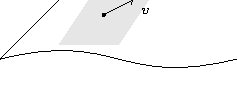
\includegraphics[width=\textwidth]{tangent.pdf}}
%   \end{minipage}\hfill%
%   \hfill\begin{minipage}{.5\textwidth}
%       \boxed{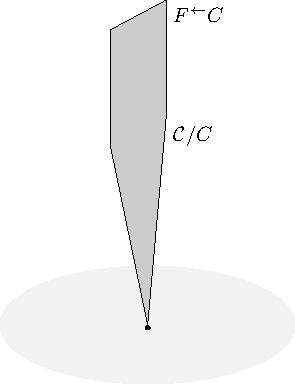
\includegraphics[scale=.5]{slice.pdf}}
%   \end{minipage}
% \end{frame}
%
%
%
%
%
%
%
%
%
\begin{frame}{Tangent cohesion}
  \begin{prop}
    Functor $\delta\colon T\clC\to \clC$ = domain projection. Has left adjoint the functor $\Omega\colon \clC\to T\clC$ that is also a \emph{section} for $q$.
    
    \onslide<+->
    $\Omega(A)$ = the complex of \alert{differential forms} on an internal abelian group $A\in \text{Ab}(\clC/X)$.
  \end{prop}
  
  \onslide<+->
  \vspace*{\fill}
  In classical differential geometry a leading theorem is that the co/tangent bundle to a smooth manifold is  itself a smooth manifold. Here we can prove that
  
  \onslide<+->
  \vspace*{\fill}
  \begin{myblock}{Fact}
    The tangent category to a cohesive topos is itself a cohesive topos.
  \end{myblock}
\end{frame}
%
%
%
%
%
%
%
% \begin{frame}{Infinitesimal cohesion}
%   \begin{variableblock}{}{bg=red!10, fg=black}{bg=red!10, fg=blue}
%     Neighbourhoods of some spaces are ``infintesimally extended around a single (global) point''. Cohesive structure can be refined to capture this phenomenon.
%   \end{variableblock}
% \end{frame}
% %
%
%
%
%
%
%
\begin{frame}{Infinitesimal cohesion}
  Let $\clH$ be cohesive. An \alert{infinitesimal thickening} of $\clH$ is a new cohesive topos $\thH$ linked to the previous by a quadruple of adjoints
  \[
  \xymatrix@R=1.5cm{
  \clH
  \ar@{^{(}->}@<-18pt>[d]_{(i_! \dashv i^* \dashv i_! \dashv i^!)}
  \only<3->{\ar@{^{(}->}@<6pt>[d]}
  \\
  \ar@[white]@<-18pt>[u]
  \only<2->{\ar@<6pt>[u]}
  \only<4->{\ar@<-18pt>[u]}
  \thH
  }
  \]
  
  \vspace*{\fill}
  \onslide<5->such that $i_*, i_!$ are fully faithful and $i_!$ commutes with finite products.
  
  If such a structure exists, $\clH$ ``exhibits \textbf{infinitesimal} cohesion''.
  \onslide<6->
  \begin{variableblock}{}{bg=red!10, fg=black}{bg=red!10, fg=blue}
    \small Neighbourhoods of some spaces are ``infintesimally extended around a single (global) point''. Cohesive structure can be refined to capture this phenomenon.
  \end{variableblock}
\end{frame}
%
%
%
%
%
%
%
\begin{frame}{Infinitesimal cohesion}
  \begin{itemize}
    \item<+-> The cohesion exhibited by $\thH$ \alert{factors through} that of $\clH$, in that
    \[
    (\Pi_{\thH} \dashv \disc_{\thH} \dashv \Gamma_{\thH})
    \colon
    \xymatrix@C=2cm{
    \thH \ar@<-8pt>[r]_{\th{i^!}} \ar@{<-}[r]|{i_*} \ar@<8pt>[r]^{i^*} &
    \clH \ar@<-8pt>[r]_\Gamma \ar@{<-}[r]|{\disc} \ar@<8pt>[r]^\Pi &
    \Set
    }
    \]
    \item<+-> \textbf{Infinitesimal} cohesion describes formally infinitesimally extended neighbourhoods: if the functor $i^*$ is interpreted as a \alert{contraction} of a fat point onto its singleton, then $X\in \thH$ is infinitesimal if $i^*(X)\cong *$. \onslide<+->This motivates the fact that
    \[
    \thH(*,X)\cong \thH(i_!(*),X)\cong \clH(*,i^*(X))\cong \clH(*,*)\cong *
    \]
    so that $\clH$ sees $X$ as a  ``small neighbourhood concentrated around a single point $*_X$''.
  \end{itemize}
\end{frame}
%
%
%
%
%
%
%
\begin{frame}{Higher order cohesion: jet spaces}
  Most examples of infinitesimal cohesions come equipped with an infinite chain of thickening approximations.
  
  \onslide<+->
  \begin{center}
    Consider the \alert{infinitesimal shape modality} $\Im := i_\ast i^\ast$\\
    (it comes equipped with other two adjoints, $\Re \dashv \Im \dashv \&$)\footnote{This is the same general fact inducing $\shape\dashv\flat\dashv\sharp$ adjunction.}
  \end{center}
  \onslide<+->
  In several cases (like \alert{smooth manifolds}) we have a \textbf{chain} of infinitesimal thickenings
  \[
  \xymatrix@C=1.25cm{
  \thH_0 \quadruple{(0)} & \thH_1 \quadruple{(1)} & \thH_2 \quadruple{(2)} & \quad\cdots\quad \quadruple{\#} & \thH_\infty \quadruple{(\infty)} & \clH
  }
  \]
  \onslide<+->
  here we speak of a \alert{sequence of orders of differential structures}.
\end{frame}
%
%
%
%
%
%
%
\begin{frame}{Higher order cohesion: jet spaces}
  Each of these approximations comes equipped with an \emph{order $k$ infinitesimal shape} modality $\Im^{(k)}X$ in a sequence
  \[
  X \to \Im X = \Im^{(0)}X \to \Im^{(1)}X\to \Im^{(2)}X \to\cdots
  \]
  \onslide<+->
  \textbf{Example}: Every cohesive topos exhibits infinitesimal cohesion via its \textbf{tangent} cohesive topos. This cohesion extends to any order of differential structure (``cohesive jet spaces'').
\end{frame}

\begin{frame}
  One can go \alert{way} further, but the terminology becomes pretty dire:
  \begin{center}
    \includegraphics[width=\textwidth]{nlab.png}
  \end{center}
  \begin{flushright}
    [DCCT170811], 1040 pages of Hegel-ish mathematics
  \end{flushright}
  uses axiomatic cohesion of $\infty$-toposes to axiomatise string theory. \onslide<2-> With Aufhebung.
\end{frame}

\begin{frame}{Supergeometry: rheonomy}
  We can speak of \alert{supergeometry} and show that certain categories of supersmooth manifolds exhibit cohesion (but not over $\Set$\dots):
  \[
  \xymatrix{
  \text{SuperSmoothS}
  \ar@<12pt>@{<-}[d]^c
  \ar@<-4pt>@{<-}[d]|d
  \ar@<4pt>[d]|\Gamma
  \ar@<-12pt>[d]_\Pi\\
  \text{SuperS}
  }
  \]
  The quadruple of adjoints generates the triple
  \[\rightrightarrows
  \quad \dashv \quad
  \rightsquigarrow
  \quad \dashv \quad
  \textrm{Rh}\]
  (in some sense ``fermions'' $\dashv$ ``bosons'')
\end{frame}
%
%
%
%
%
%
%
\begin{frame}{Supergeometry: rheonomy}
  There is a ``quadruple-to-triple''pattern here:
  \def\fisrt{\text{cohesion}}
  \def\secnod{\text{elasticity}}
  \def\trhid{\text{solidity}}
  \begin{center}
    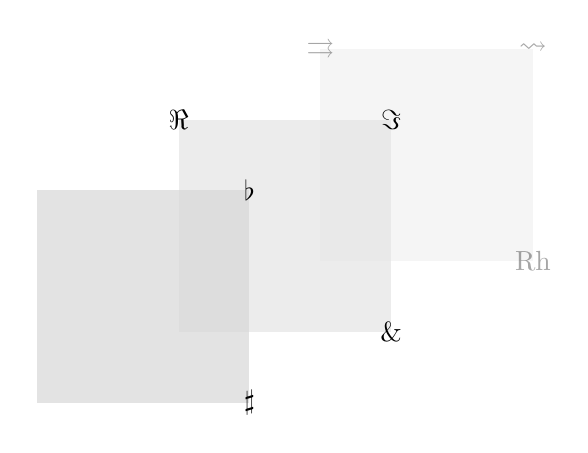
\begin{tikzpicture}[scale=.9]
      \begin{scope}[xshift=4cm,yshift=2cm, opacity=.35]
        \fill[fill opacity=.75,gray!10] (0,0) rectangle (3,3);
        \node (squig) at (0,0) {};
        \node (two) at (0,3) {$\rightrightarrows$};
        \node (squig2) at (3,3) {$\rightsquigarrow$};
        \node (rh) at (3,0) {$\textrm{Rh}$};
        \node (fisrt) at ($(squig)!.5!(squig2)$) {$\trhid$};
      \end{scope}
      \begin{scope}[xshift=2cm,yshift=1cm]
        \fill[fill opacity=.75,gray!20] (0,0) rectangle (3,3);
        \node (im) at (0,0) {};
        \node (re) at (0,3) {$\Re$};
        \node (im2) at (3,3) {$\Im$};
        \node (and) at (3,0) {$\&$};
        \node (fisrt) at ($(im)!.5!(im2)$) {$\secnod$};
      \end{scope}
      \fill[fill opacity=.75,gray!30] (0,0) rectangle (3,3);
      \node (flat) at (0,0) {};
      \node (shape) at (0,3) {$\shape$};
      \node (flat2) at (3,3) {$\flat$};
      \node (sharp) at (3,0) {$\sharp$};
      \node (fisrt) at ($(flat)!.5!(flat2)$) {$\fisrt$};
    \end{tikzpicture}
  \end{center}
\end{frame}
%
%
%
%
%
%
%
\begin{frame}{de Rham cohomology in cohesion}
  \begin{itemize}
    \item Let $\clH$ be a cohesive topos, and $0\to A$ a pointed object (e.g. an internal abelian group); then, $A$ fits into a pullback square 
    \[\xymatrix{\flat_\text{dR}A\ar[r]\ar[d]\ar@{}[dr]|\lrcorner & \flat A \ar[d]\\ 
    0 \ar[r] & A }\]
    where $\flat_\text{dR}A$ is the \alert{object of coefficients} for de Rham cohomology.
    \item Let $X\in\clH$ any object; we define $\shape_\text{dR}X$ to be the pushout
    \[\xymatrix{
    X \ar[r]\ar[d]& 0\ar[d] \\
    \shape X \ar[r] & \shape_\text{dR}X
    }\]
    where $\shape_\text{dR}X$ is the \alert{de Rham object} associated to $X$.
  \end{itemize}
\end{frame}
%
%
%
%
%
%
\begin{frame}{de Rham cohomology in cohesion}
  There is an adjunction 
  \[
  \xymatrix{
  {*/\clH}\ar@<5pt>[rr]^{\flat_\text{dR}} &&\ar@<5pt>[ll]^{\shape_\text{dR}} \clH
  } 
  \]
  The mapping space $*/\clH(\shape_\text{dR}X,A)\cong \clH(X, \flat_\text{dR}A)$ is called the \alert{}{de Rham space} of $X$ with coefficients in $A$ and denoted $\mathbf{H}^0_\text{dR}(X,A)$.
\end{frame}
%
%
%
%
%
\begin{frame}{de Rham cohomology in cohesion}
  Consider the pullback defining $\flat_\text{dR}A$ and apply the limit-preserving functor $\clH(X,-)$: the square
  \[\xymatrix{\clH(X,\flat_\text{dR}A)\ar[r]\ar[d]\ar@{}[dr]|\lrcorner & \clH(X,\flat A) \ar[d]\\ 
  0 \ar[r] & \clH(X,A) }\]
  remains a pullback and the object $\clH(X,\flat A)$ identifies to \alert{$A$-valued differential forms}, and the maps $X \to \flat_\text{dR}A$ are the \alert{flat} ones: under the $\shape\dashv \flat$ adjunction, a map $X\to \flat A$ mates to a smooth map $\shape X \to A$, corresponding to a square
  $
  \begin{smallmatrix}
    X &\to & 0 \\
    \downarrow && \downarrow \\
    \shape X &\to& A
  \end{smallmatrix}
  $
\end{frame}
%
%
%
%
%
%
%
%
\begin{frame}{(minimal) Bibliography}
  \centering
  \footnotesize
  \begin{minipage}{.85\textwidth}
    \begin{itemize}
      \item[Law1] Lawvere, F. William. \emph{Axiomatic cohesion}. Theory Appl. Categ 19.3 (2007): 41-49.
      \item[Law2] Lawvere, F. William. \emph{Categorical dynamics}. Topos theoretic methods in geometry 30 (1979): 1-28.
      \item[Law3] Lawvere, F. William. \emph{Toposes of laws of motion}. American Mathematical Society, Transcript from video, Montreal-September 27 (1997): 1997.
      \item[Urs] Schreiber, Urs. \emph{Differential cohomology in a cohesive infinity-topos}. arXiv:1310.7930 (2013).
      \item[Men] Menni, Matias. \emph{Continuous cohesion over sets}. Theory and Applications of Categories 29.20 (2014): 542-568.
      \item[MLM] MacLane, Saunders, and Ieke Moerdijk. \emph{Sheaves in geometry and logic: A first introduction to topos theory}. Springer Science \& Business Media, 2012.
    \end{itemize}
  \end{minipage}
\end{frame}  
\end{document}